\documentclass[12pt]{article}

\usepackage{sbc-template}
\usepackage{graphicx,url}
\usepackage{float}
\usepackage[brazil]{babel}   
%\usepackage[latin1]{inputenc}  
\usepackage[utf8]{inputenc}  
\usepackage{url}

\usepackage{xcolor}
% Definindo novas cores
\definecolor{verde}{rgb}{0.25,0.5,0.35}
\definecolor{jpurple}{rgb}{0.5,0,0.35}
% Configurando layout para mostrar codigos Java
\usepackage{listings}

\bibliographystyle{ieeetr}

\definecolor{lightgray}{rgb}{.9,.9,.9}
\definecolor{darkgray}{rgb}{.4,.4,.4}
\definecolor{purple}{rgb}{0.65, 0.12, 0.82}

\lstdefinelanguage{JavaScript}{
	keywords={typeof, new, true, false, catch, function, return, null, catch, switch, var, if, in, while, do, else, case, break},
	keywordstyle=\color{blue}\bfseries,
	ndkeywords={class, export, boolean, throw, implements, import, this},
	ndkeywordstyle=\color{darkgray}\bfseries,
	identifierstyle=\color{black},
	sensitive=false,
	comment=[l]{//},
	morecomment=[s]{/*}{*/},
	commentstyle=\color{purple}\ttfamily,
	stringstyle=\color{red}\ttfamily,
	morestring=[b]',
	morestring=[b]"
}

\lstset{
	language=JavaScript,
	backgroundcolor=\color{lightgray},
	extendedchars=true,
	basicstyle=\footnotesize\ttfamily,
	showstringspaces=false,
	showspaces=false,
	numbers=left,
	numberstyle=\footnotesize,
	numbersep=9pt,
	tabsize=1,
	breaklines=true,
	showtabs=false,
	captionpos=b
}

\lstset{
	language=Java,
	basicstyle=\ttfamily\small, 
	keywordstyle=\color{jpurple}\bfseries,
	stringstyle=\color{red},
	commentstyle=\color{verde},
	morecomment=[s][\color{blue}]{/**}{*/},
	extendedchars=true, 
	showspaces=false, 
	showstringspaces=false, 
	numbers=left,
	numberstyle=\tiny,
	breaklines=true, 
	backgroundcolor=\color{cyan!10}, 
	breakautoindent=true, 
	captionpos=b,
	xleftmargin=0pt,
	tabsize=4
}
\pagestyle{empty}
     
\sloppy
	\title{Web Service de Consulta de CEP e Rastreamento de Encomendas dos Correios  \\ Exercício Computacional I - Sistemas Distribuídos}

\author{Rafael Gonçalves de Oliveira Viana\inst{1} \\\vspace*{10pt} \normalsize  \today{} }


\address{Sistemas de Informação -- Universidade Federal do Mato Grosso do Sul
	(UFMS)\\
  	Caixa Postal 79400-000 -- Coxim -- MS -- Brazil
  \email{rafael.viana@aluno.ufms.br}
}

\begin{document} 

\maketitle

     
\begin{resumo} 	
  Este relatório introduz a arquitetura de um \textit{Web Service} assim como seus componentes, o mesmo relata como foi implementado um Web Server que possui uma página web e serviços para busca de cidade e bairro através do CEP e rastreamento de encomendas dos correios.
\end{resumo}



\section{Introdução}
  Com a disseminação de dispositivos com conexão a Internet na sociedade atual, houvesse a necessidade de criar/gerenciar serviços web, estes necessarios para atender as mais diversas funções como exemplo, salas de bate-papo, e-commerces e serviços meteorológicos.
  
  Este relatório apresenta brevemente a arquitetura de um \textit{Web Service} e como foi implementado, serviços de consulta de cidade e barrio através do CEP e rastreamento de encomendas dos correios, juntamente com uma página web oferecendo uma interface para os serviços disponíveis.
  
  O código deste relatório esta em sua totalidade no endereço http://github.com/rafaelgov95/SD/Projeto-Correios-CEP, e o mesmo pode ser reutilizado sobre a licença MIT.
\section{Web Service}
Webservice é uma solução utilizada na integração de sistemas e na comunicação entre aplicações diferentes, como pode ser objservado na figura \ref{wbs}, um \textit{Data Server}, disponibiliza serviços para os mais diversos tipos de dispositivos, em diferentes formatos de objetos.

Com está tecnologia é possível que novas aplicações possam interagir com aquelas que já existem e que sistemas desenvolvidos em plataformas diferentes sejam compatíveis. 
 \cite{webservece}.
\begin{figure}[H]
	\centering
	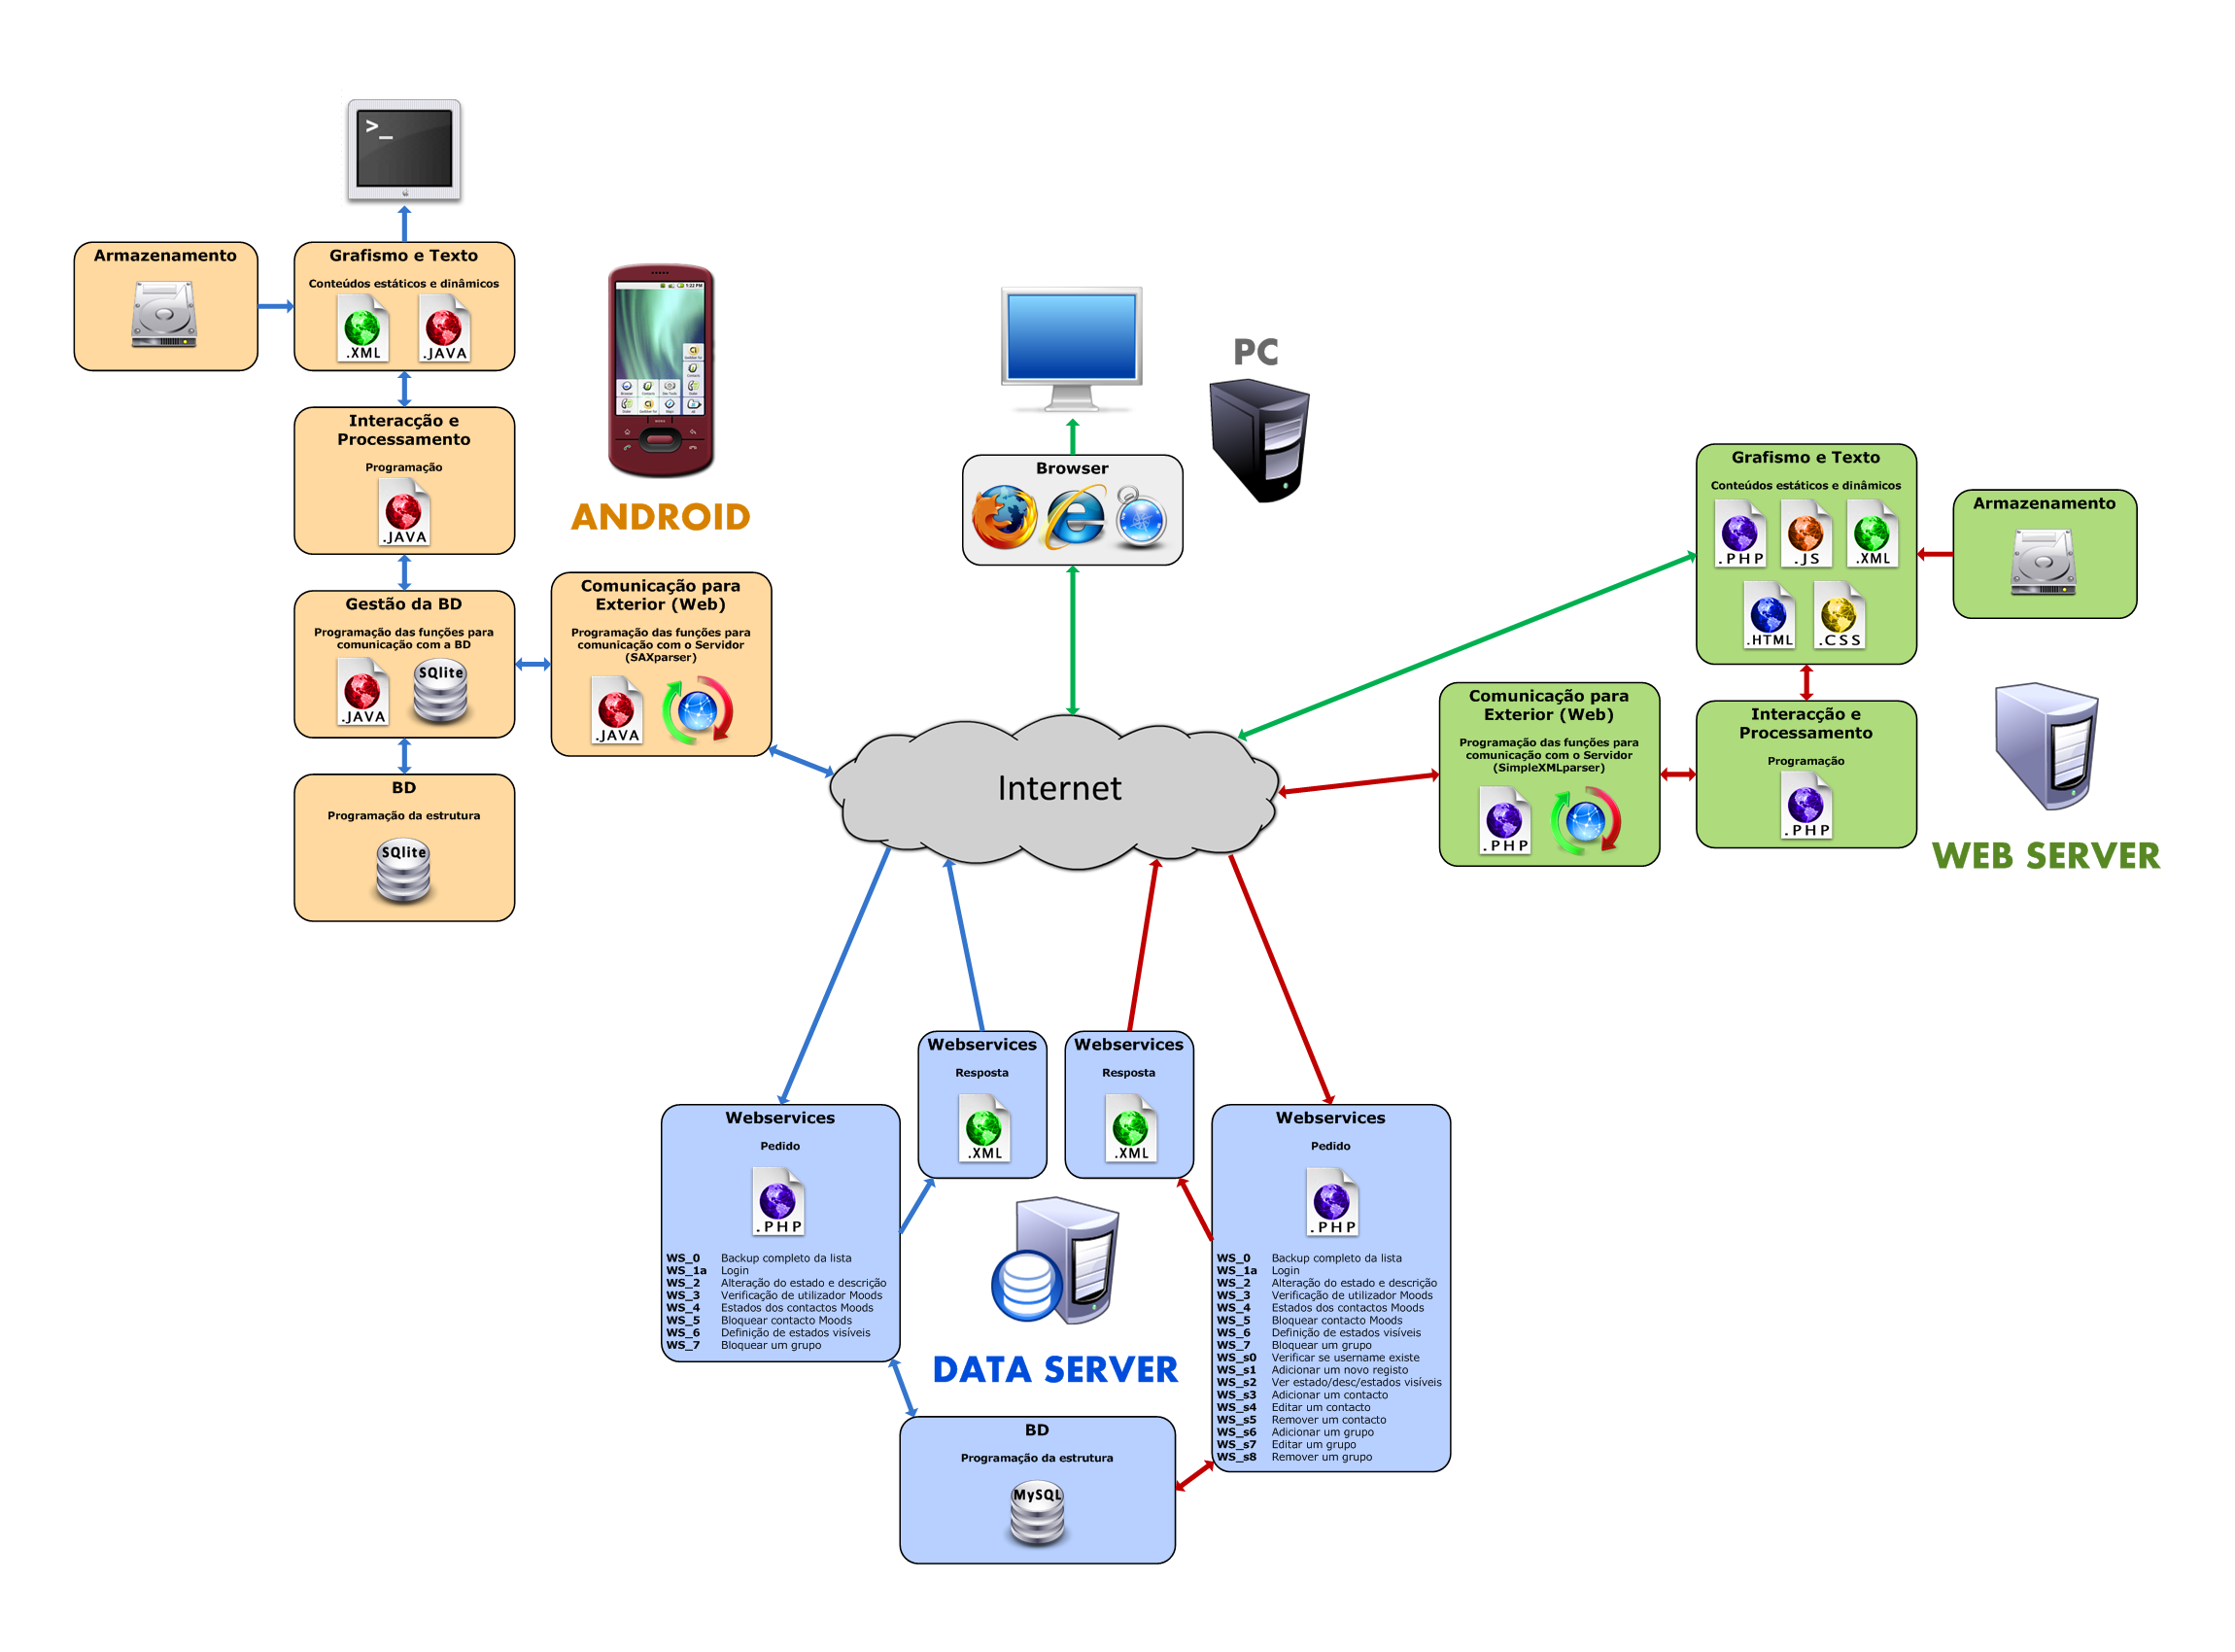
\includegraphics[scale=0.14]{Imagens/webservice.png}
	\caption{Sistema implantando, fornecendo serviços para PCs, dispositivos móveis e outros web servers.}
	\label{wbs}
\end{figure} 


\subsection{Componentes de um \textit{Web Service}}
Ao longo dos últimos anos, diversas tecnologias emergiram como padrões mundiais que constituem o núcleo da tecnologia de serviços da Web de hoje. Algumas destas tecnologias e suas caracteristicas são demostradas abaixo.


\subsubsection{WSDL - \textit{Web Services Description Language} }
O WSDL é um idioma baseado em XML para descrever os serviços da Web e como acessá-los.

\begin{enumerate}
	\item É um protocolo baseado em XML, para troca de informações em ambientes descentralizados e distribuídos.
	\item É o formato padrão para descrever um serviço web.
	\item Descreve como acessar um serviço da Web e quais as operações que ele executará.
	\item Descrever como se relacionar com serviços baseados em XML.
	\item É o idioma que UDDI utiliza.
	
\end{enumerate}

\subsubsection{SOAP - \textit{Simple Object Access Protocol}}

O SOAP é um protocolo baseado em XML para trocar informações entre computadores.

O mesmo não está vinculado a nenhum protocolo de transporte específico. Na verdade, você pode usar SOAP via HTTP, SMTP, FTP ou BEEP. 
Algumas caracteriscas estão presentes no SOAP elas são:
\begin{enumerate}
	\item Será desenvolvido como um padrão W3C.
	\item Protocolo de comunicação.
	\item Comunicação entre aplicativos.
	\item Formato para enviar mensagens.
	\item Projetado para se comunicar via Internet.
	\item Independente da plataforma.
	\item Independente da linguagem.
	\item Permite que você percorra os firewalls.
\end{enumerate}
\subsubsection{REST - \textit{Representation State Transfer}}
É uma arquitetura criada para ser mais simples de se usar que o SOAP. Pode ser usado em vários formatos de texto, como CSV (Comma-separated Values), RSS (Really Simple Syndication), JSON e YAML. Porém, só pode ser utilizado com o protocolo HTTP/HTTPS, por exemplo utilizando os métodos GET, POST, PUT e DELETE. 

\begin{enumerate}
	\item Melhor curva de aprendizado.
	\item Mensagens menores e mais eficientes como o formato JSON comparado com XML.
	\item Os dados podem ser colocados em cache, retornando sempre a mesma resposta para a mesma requisição.
	\item Mais rápido pois precisa de menos processamento que o SOAP.
\end{enumerate}
 
 
 \subsection {Principais Serviço de Transporte de um Web Service}Os protocolos da camada inferior ficam responsáveis pelo transporte de serviços. Essa camada é responsável por transportar como exemplo mensagens XML e JSON entre dois computadores.
 \begin{enumerate}
 	\item \textbf{Hyper Text Transfer Protocol (HTTP):}
 	É a opção mais popular para o transporte de serviços. O HTTP é simples, estável e amplamente implantado. Além disso, a maioria dos firewalls permitem o tráfego HTTP. Isso permite que mensagens REST ou SOAP se mostrem como mensagens HTTP. Isso é bom se você quiser integrar aplicativos remotos, mas eleva uma série de preocupações de segurança.
 	\item \textbf{Bloqueia o protocolo de troca extensível (BEEP)}
 	Esta é uma alternativa promissora para o HTTP. O BEEP é uma nova estrutura da Task Force de Engenharia da Internet (IETF) para a construção de novos protocolos.
 \end{enumerate}
 
\section{Qual Arquitetura de Web Service utilizar}
Para poder identificar qual arquitetura utilizar de \textit{Web Service}, deve-se examinar os papéis individuais de cada ator no contexto, e também a pilha emergente de protocolo que o mesmo pretende utilizar.
O mesmo pode ser publicado na intranet ou na Internet, provendo três possiveis formatos de serviços: Provedor de Serviço, Solicitante de Serviço e o Registro de Serviço.
Para mais detalhes desta sessão incentivo consultar a referências \cite{tutorial}. 

\begin{enumerate}
	\item \textbf{Provedor de serviço:}
	Fornece serviços web. O provedor de serviços implementa o serviço e disponibiliza-o na Internet ou intranet.
	\item \textbf{Solicitante de Serviço:}
	Este é um consumidor do serviço web. O solicitante utiliza um serviço da Web existente abrindo uma conexão de rede e enviando uma solicitação XML.
	\item \textbf{Registro de serviço:}
	Este é um diretório de serviços logicamente centralizado. O registro fornece um lugar central onde os desenvolvedores podem publicar novos serviços ou encontrar os existentes. Ele serve como centro de compensação centralizado para empresas e seus serviços.
\end{enumerate}

Outro modo de identificar qual arquitetura utilizar, é examinar a pilha emergente de protocolo que pretende utilizar. Cada dia existe mais tipos de protocolos porém existem 4 tipo que se destacam: Serviço de Transporte - "FTP", Mensgens "XML", Descrição de Serviço "WSDL"  e Descoberta de Serviço "UDDI".

	Podemos observar na figura \ref{wbss}, a pilha de soluções com a pilha de tecnologia correspondente para cada camada. 
\begin{enumerate}
	\item \textbf{Descoberta do serviço:}
	Responsável por centralizar os serviços em um registro comum e fornecer funcionalidades fáceis de publicação/pesquisa. Atualmente, a descoberta do serviço é tratada através de Descrição Universal, Descoberta e Integração (UDDI).
	\item \textbf{Descrição do Serviço:}
	Responsável por descrever a interface pública para um serviço web específico. Atualmente, a descrição do serviço é tratada através do Web Service Description Language (WSDL).
	\item \textbf{Mensagens XML:}
	Responsável por codificar mensagens em um formato XML comum para que as mensagens possam ser entendidas em cada uma das extremidades. Atualmente, esta camada inclui XML-RPC e SOAP.
	\item \textbf{Serviço de transporte:}
	 Responsável pelo transporte de mensagens entre aplicativos. Atualmente, esta camada inclui o protocolo de transporte de hipertexto (HTTP), protocolo de transferência de correio simples (SMTP), protocolo de transferência de arquivos (FTP) e protocolos mais recentes, como o protocolo de intercâmbio extensível de blocos (BEEP).


\end{enumerate}
\begin{figure}[H]
	\centering
	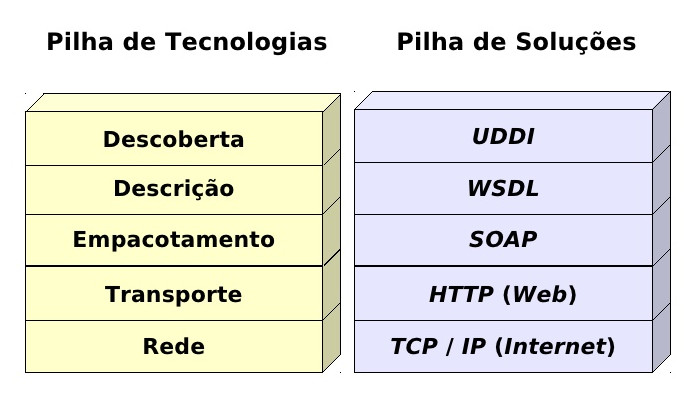
\includegraphics[scale=0.5]{Imagens/pilhat.jpg}
	\caption{Pilha de protocolo de transporte e suas tecnologias. }
	\label{wbss}
\end{figure}

\section{Metodologia}
Nesta sessão relato como foi o desenvolvimento e a implantação de um \textit{Web Service} em um \textit{Web Server} que promove serviços de busca de CEPs e rastreamento de encomendas dos correios, utilizando uma página web como interface para consultas.
 
\subsection{Web Server}
	O \textit{Web Server} foi implementado utilizando o NodeJS com o framework ExpressJs, onde se cria um ambiente de desenvolvimento para criação de serviços web.
	\begin{quote}
	O Node.js usa um modelo de E/S não bloqueante, que o torna leve e eficiente. O ecossistema de pacotes Node.js, npm , é o maior ecossistema de bibliotecas de código aberto do mundo \cite{nodejs}.
	\end{quote}
	\begin{quote}
	O Express é um framework para aplicativo da web do Node.js mínimo e flexível que fornece um conjunto robusto de recursos para aplicativos web e móvel \cite{expressjs}.
	\end{quote}

\subsection{Web Service de Busca de CEP}
	A busca de cidade e bairro pelo CEP está sendo tercerizada por um \textit{Web Service}, que prove este serviço com base nos dados de seu banco de dados, nos mais diversos tipos de empacotamento. Esses serviços são fornecidos pela empresa \textit{VIACEP}, o site da mesma é https://viacep.com.br/.

	Uma página web RafaelBuscas foi desenvolvida utilizando o framework Angular, a mesma consome o serviço de cep, no formato JSON fornecido pelos servidores da \textit{VIACEP}.
	
	A url do serviço web da VIACEP consumida pela página RafaelBuscas, está disponível http://viacep.com.br/ws/CodigoCEP/json/, o mesmo encaminha uma requisição HTTP-GET, com o código do CEP, retornando uma resposta em JSON, com as informações do CEP (Localização, Bairro, Código IBGE, GIA entre outras), conforme a figura \ref{c33}, para mais informações sobre requisições nos servidores da \textit{VIACEP} consultar a referência \cite{viacep}. 
	 \begin{figure}[H]
		\centering
		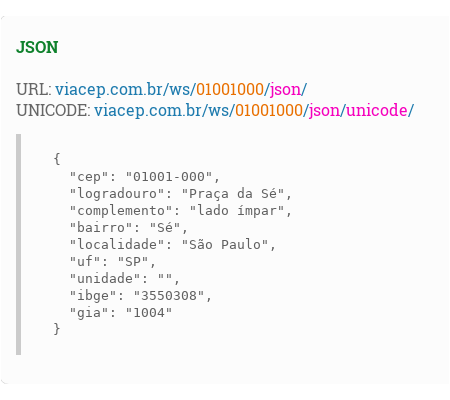
\includegraphics[scale=0.6]{Imagens/via.png}
		\caption{Modelo de requisição HTTP-GET e seu retorno.}
		\label{c33}
	\end{figure}
\subsection{Web Service Encomendas dos Correios}
	O rastreiamento por encomendas dos correios, dispõe de duas tecnologias diferentes de empacotamento, fornecida pelos Correios. A primeira utiliza a tecnologia SOAP, e outra alternativa é utilizar uma requisição REST HTTP-POST, para obter uma requisição da página oficial dos correios e após receber a resposta em um objeto HTML, e realizado um parsear na resposta.
\subsubsection{Serviço de Rastreamento Encomenda via SOAP}
O WSDL dos correios que fornece recursos para os serviços de requisição SOAP,o serviço de rastreamento de encomendas dos correios via SOAP é gratuito.

A Url "http://webservice.correios.com.br:80/service/rastro" é o endereço do \textit{Web Service} e não do WDSL, o webservice espera uma mensagem SOAP como na Listing \ref{c1} a mesma deve ser assinada com cabeçalhos HTTP no formato "Content-Type", "text/xml".
\lstset{
	language=xml,
	tabsize=3,
	%frame=lines,
	caption=Código XML SOAP para requisição de localização de pacote,
	label=c1,
	frame=shadowbox,
	rulesepcolor=\color{gray},
	xleftmargin=20pt,
	framexleftmargin=15pt,
	keywordstyle=\color{blue}\bf,
	commentstyle=\color{OliveGreen},
	stringstyle=\color{red},
	numbers=left,
	numberstyle=\tiny,
	numbersep=5pt,
	breaklines=true,
	showstringspaces=false,
	basicstyle=\footnotesize,
	emph={food,name,price},emphstyle={\color{magenta}}}
\lstinputlisting{Codigo/codigo1.xml}

Utilizando a linguagem Java e a biblioteca \textit{javax.xml.soap}, houve o envio de requisição SOAP com a mensagem da Listing \ref{c1} para o \textit{Web Service} de rastreamento de encomendas, fornecido pelos correios para mais informações referente a API de serviços dos correios, incentivo consultar a referência \cite{correios}.

O retorno da requisição é um código XML, contendo a resposta da requisição, como demostrano na Listing \ref{c2}.
 \lstset{
 	language=xml,
 	tabsize=1,
 	%frame=lines,
 	caption=Resposta da Requisição SOAP,
 	label=c2,
 	frame=shadowbox,
 	rulesepcolor=\color{gray},
 	xleftmargin=20pt,
 	framexleftmargin=15pt,
 	keywordstyle=\color{blue}\bf,
 	commentstyle=\color{OliveGreen},
 	stringstyle=\color{red},
 	numbers=left,
 	numberstyle=\tiny,
 	numbersep=5pt,
 	breaklines=true,
 	showstringspaces=false,
 	basicstyle=\footnotesize,
 	emph={food,name,price},emphstyle={\color{magenta}}}
 \lstinputlisting{Codigo/codigo2.xml}
 Esse serviço disponibilizado pelos correios apesar de ser gratuito, somente retorna a última atualização do objeto como demostrado na Listing \ref{c2}.
\subsubsection{Serviço de Rastreamento de Encomendas alternativo utilizando Crawling na Página dos Correios}

	Existe um serviço disponível na página dos correios para rastreamento de encomendas, onde é possivel realizar um crawling na página, para obter um objetivo HTML, contendo as informações da encomenda buscada.
	
	O serviço está disponível na url "http://www2.correios.com.br/sistemas/rastreamento/", a imagem \ref{c1} demostra como pode-se utilizar a ferramenta \textit{Postman}, para realizar uma requisição REST HTTP-POST, direto para página de rastreamento, com objetivo de extrair informações da mesma.
	
	 \begin{figure}[H]
	 	\centering
	 	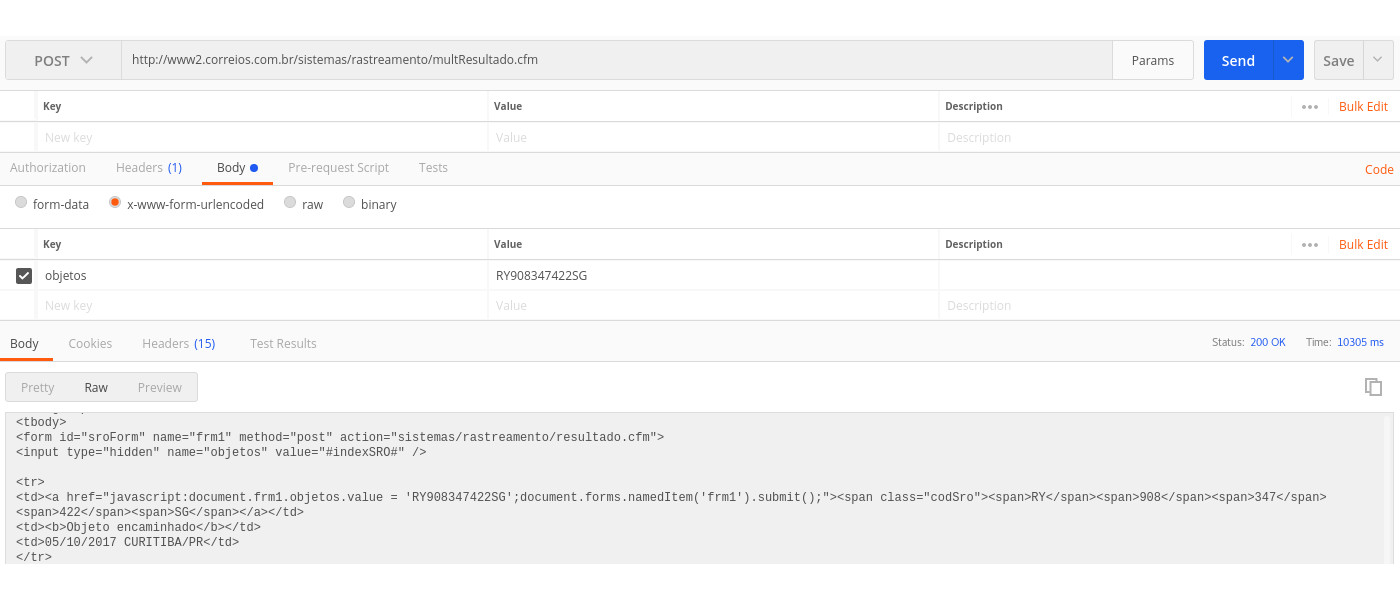
\includegraphics[scale=0.3]{Imagens/c1.jpg}
	 	\caption{Postman realizando um requsição REST HTTP-POST.}
	 	\label{c1}
	 \end{figure}
	
	Para consumir o serviço da página dos correios, primeiramente, foi desenvolvivdo um \textit{Web Service} com NodeJs e o framework ExpressJs, junto com a biblioteca request-promise para requisição JavaScript e a biblioteca cheerio para realizar o parse das tags "tr'' e ''td'' (onde estão as informações da encomenda, demostrado na figura  \ref{c1}, no campo body do response) do HTML.
	
	Na Listing \ref{c3} consta um método que realiza uma requisição REST - HTTP-POST no \textit{Web Server} da página web.
	
	\medskip
	\begin{lstlisting}[caption=Criando Requisição em Java Script,label=c3]
	request: function (req) {
	var correios = {
	uri: "http://www2.correios.com.br/sistemas/rastreamento/multResultado.cfm",
	form: {
	objetos: req.params.code
	},
	method: 'POST',
	headers: {}
	};
		response = requestPromise(correios);
		console.log(response)
		return response
	}	
	\end{lstlisting}
	Após a requisição da Listing \ref{c3}, teremos uma variável, contendo todo o HTML da página web, que foi obtida pela requsição.
	
	Utilizando a função na Listing \ref{c4}, realizamos um parse no HTML, com o objetivo de extrair as informações referente a encomenda.
	
	O parse percorre a tabela e extrai, algumas informações (código, localidade, data, situação) criando um objeto JSON, com as informações de rastreamento obtidas, que será consumido pela página web RafaelBuscas.
	
	Realizando uma requisição através da página RafaelBuscas ou utilizando diretamente a url http://rafaelbuscas.ddns.bet/json/"codigo-de-rastreamento", primeiramente a requisição é recebida pelo \textit{Web Service} (que está aguardando na rota da url acima), onde o mesmo envia uma requisição HTTP-POST, para a página de rastreamento dos correios com o código de encomenda fornecido, após o parse realizado as informações são encaminhandas em um objeto JSON, como resposta para requisição inicial.   
	\medskip
	\begin{lstlisting}[caption=Criando um Crawling para parsar as tags,label=c4]
	
	parser: function (data) {
		var $ = cheerio.load(data);
		var objetos = [];
		var tableObjetos = $('table').find('tr');
		$(tableObjetos).map(function(key, objeto){
			objeto  = $(objeto).children('td').map(function (key, field) {
				return $(field).text();
			}).toArray();
			if (objeto[0]) {
				
				var rastreio = {
					codigo  : null,
					situacao: null,
					local   : null,
					data    : null
				};
				
				rastreio.codigo     = objeto[0].trim();
				if (objeto[2]) {
					rastreio.situacao   = objeto[1];
					rastreio.local      = objeto[2].substr(11, objeto[2].length).trim();
					rastreio.data       = objeto[2].substr(0,10).trim();
				} else {
					rastreio.situacao   = 'Objeto ainda nao consta no sistema'
				}
				
				objetos['rast'] = rastreio;
			}
		});
		
		return Object.assign({}, objetos);
	}
	  	\end{lstlisting}
	  	
	  	
	  	\section{Página RafaelBuscas}
	  	Para fins didaticos, os serviços de rastreamento de encomendas e buscas de cep pelo código, relatados estão disponíveis na url http://rafaelbuscas.ddns.net, a mesma possui uma página web como interface para os serviços, estes que estão hospedados em uma máquina virtual do Google Cloud.
	  	
	  	Na página inical no canto inferior, existe um input para o código do CEP ou do Rastreamento (fornecidos pelos correios).
	  	
	  	Um componente para seleção de consulta entre Cep ou Rastremamento, com o nome de ''TIPO'', deve ser marcado como CEP ou Rastreio, antes da busca (botão com uma lupa) como demostrado na Figura \ref{c2}.
	  	
	  		 \begin{figure}[H]
	  		\centering
	  		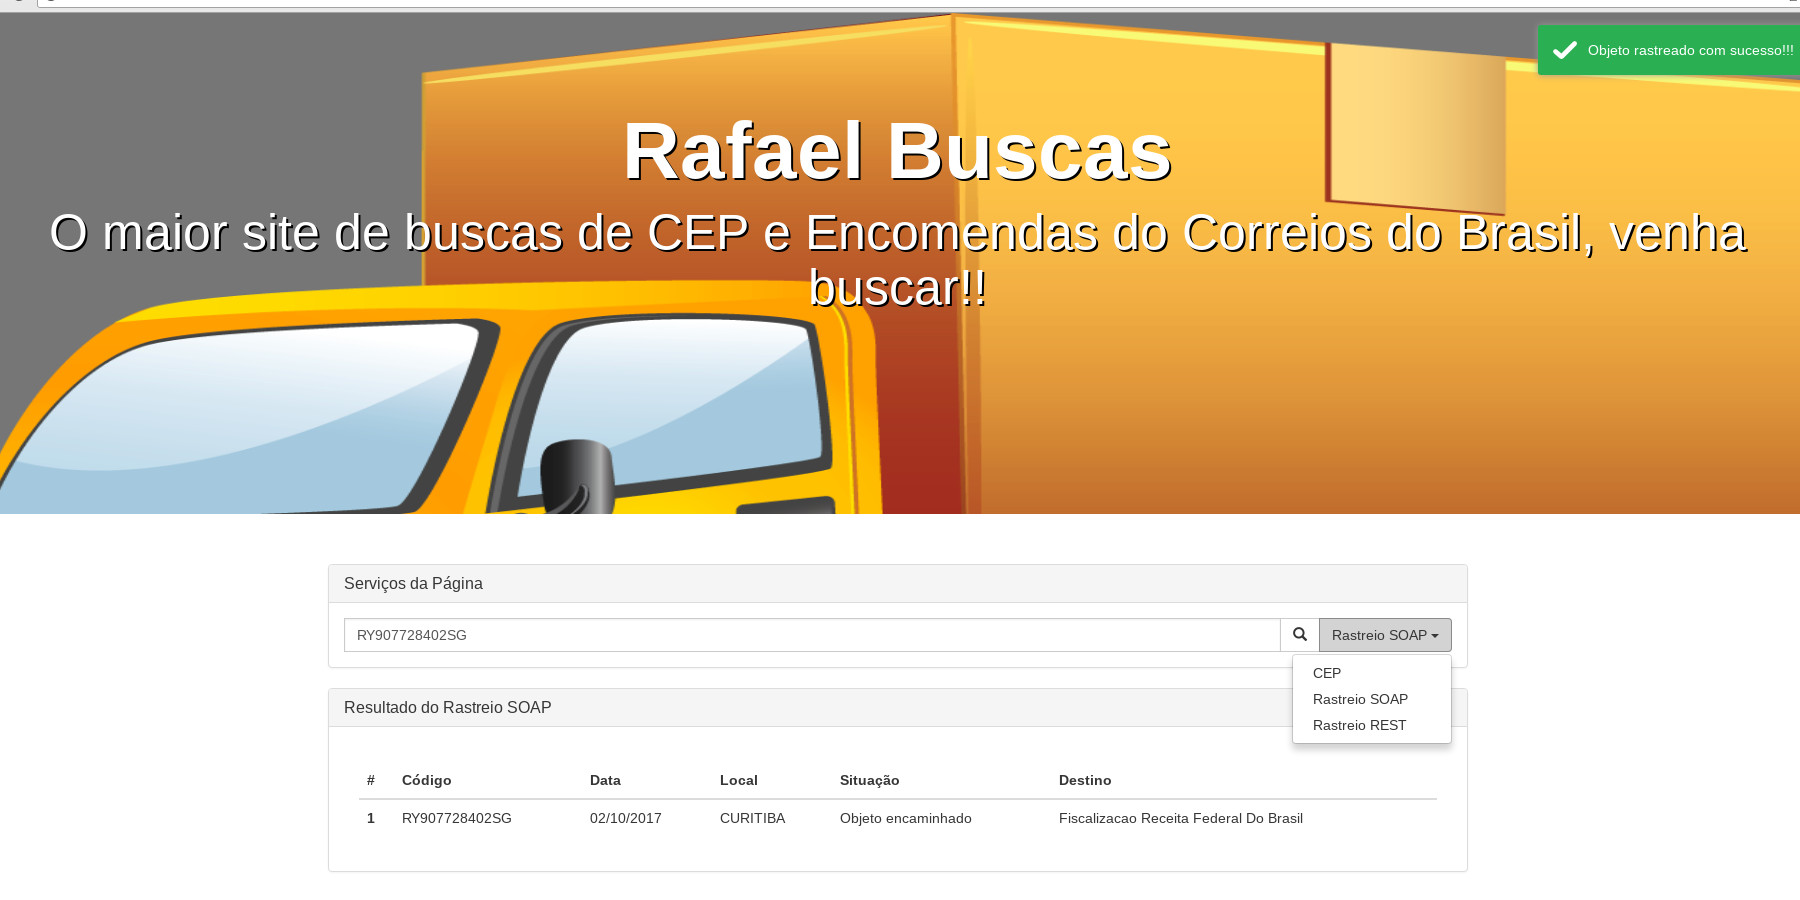
\includegraphics[scale=0.23]{Imagens/c2.jpg}
	  		\caption{Página RafaelBuscas, demostração de busca de cep.}
	  		\label{c2}
	  	\end{figure}
\section{Conclusão}
Neste relatório foi apresentado a estrutura básica de um \textit{Web Services}, e como o pŕoprio pode ser utilizado para consumir serviços de outros \textit{Web Services} disponíveis por outras empresas, outra abordagem exposta seria utilizar os mesmos para criação de um novo serviço, em seu próprio \textit{Web Server}, para atender as mais diversas necessidades, como exemplo o rastreiamento de encomendas ou obter a cidade e o bairro através de um CEP.	  	

	  \bibliography{bibli}

\end{document}


